\documentclass[11pt,table]{beamer}
\mode<presentation>
\usepackage{etex}
\usepackage{graphicx}
\usepackage{epstopdf}
\usepackage[english]{babel}
\usepackage{tabularx}
\usepackage{booktabs}
\usepackage{mathrsfs}
\usepackage{multicol}
\usepackage{bm}
\usepackage{subcaption}
\usepackage{wrapfig}
\usepackage{dcolumn}
\usepackage{threeparttable}
\usepackage{booktabs}
\usepackage{bbm}
\usepackage{amsmath,dsfont,listings}
\usepackage{amssymb}
\usepackage{rotating}
\usepackage{multirow}
\usepackage[authoryear]{natbib}
\usepackage{circledsteps}
\usepackage{tikz}
\usetikzlibrary{arrows,decorations.pathmorphing,backgrounds,fit,positioning,shapes.symbols,chains}
\setbeamertemplate{section in toc}[sections numbered]
\setbeamertemplate{caption}[numbered]

\bibliographystyle{Econometrica}

\setbeamersize{text margin right=3.5mm, text margin left=7.5mm}  % text margin
\setbeamersize{sidebar width left=0cm, sidebar width right=0mm}
\setbeamertemplate{sidebar right}{}
\setbeamertemplate{sidebar left}{}

\definecolor{text-grey}{rgb}{0.45, 0.45, 0.45} % grey text on white background
\definecolor{bg-grey}{rgb}{0.66, 0.65, 0.60} % grey background (for white text)
\definecolor{fu-blue}{RGB}{0, 51, 102} % blue text
\definecolor{fu-green}{RGB}{153, 204, 0} % green text
\definecolor{fu-red}{RGB}{204, 0, 0} % red text (used by \alert)

\setbeamertemplate{frametitle}{%
    \vskip-30pt \color{text-grey}\large%
    \begin{minipage}[b][23pt]{80.5mm}%
    \flushleft\insertframetitle%
    \end{minipage}%
}

\setbeamertemplate{navigation symbols}{} 

%%% begin title page
\setbeamertemplate{title page}{
\vskip2pt\hfill
\vskip6pt\hskip3pt

% set the title and the author
\vskip14pt
\parbox[top][1.35cm][c]{11cm}{\LARGE\color{text-grey} Econome\textcolor{red1}{tricks}: \inserttitle \\[1ex] \small \quad \\[3ex]}
\vskip11pt
\parbox[top][1.35cm][c]{11cm}{\small Trick 03: \insertsubtitle \\[2ex] \insertauthor \\[1ex]}
}
%%% end title page

%%% colors
\usecolortheme{lily}
\setbeamercolor*{normal text}{fg=black,bg=white}
\setbeamercolor*{alerted text}{fg=fu-red}
\setbeamercolor*{example text}{fg=fu-green}
\setbeamercolor*{structure}{fg=fu-blue}

\setbeamercolor*{block title}{fg=white,bg=black!50}
\setbeamercolor*{block title alerted}{fg=white,bg=black!50}
\setbeamercolor*{block title example}{fg=white,bg=black!50}

\setbeamercolor*{block body}{bg=black!10}
\setbeamercolor*{block body alerted}{bg=black!10}
\setbeamercolor*{block body example}{bg=black!10}

\setbeamercolor{bibliography entry author}{fg=fu-blue}
\setbeamercolor{bibliography entry journal}{fg=text-grey}
\setbeamercolor{item}{fg=fu-blue}
\setbeamercolor{navigation symbols}{fg=text-grey,bg=bg-grey}
%%% end colors

%%% headline
\setbeamertemplate{headline}{
\vskip30pt
}
%%% end headline

%%% footline
\newcommand{\footlinetext}{
%\insertshortinstitute, \insertshorttitle, \insertshortdate
}
\setbeamertemplate{footline}{
\vskip2pt
\hfill \raisebox{-1pt}{\usebeamertemplate***{navigation symbols}}
\hfill \insertframenumber\hspace{10pt}
\vskip4pt
}
%%% end footline

%%% settings for listings package
\lstset{extendedchars=true, showstringspaces=false, basicstyle=\footnotesize\sffamily, tabsize=2, breaklines=true, breakindent=10pt, frame=l, columns=fullflexible}
\lstset{language=Java} % this sets the syntax highlighting
\lstset{mathescape=true} % this switches on $...$ substitution in code
% enables UTF-8 in source code:
\lstset{literate={�}{{\"a}}1 {�}{{\"o}}1 {�}{{\"u}}1 {�}{{\"A}}1 {�}{{\"O}}1 {�}{{\"U}}1 {�}{\ss}1}
%%% end listings

\usepackage{concmath}
\usepackage{xcolor}
\definecolor{lightblue}{rgb}{0.8,0.85,1}
\definecolor{persianred}{rgb}{0.8, 0.2, 0.2}
\definecolor{red1}{RGB}{206, 17, 38}
\definecolor{blue1}{RGB}{16, 118, 208}
\definecolor{gray1}{RGB}{117, 115, 115}
\usepackage{hyperref}


\newtheorem{proposition}{Proposition}
\newtheorem{assumption}{Definition}

\title[]{Short guides to econometrics}
\subtitle[]{Review of Distribution Theory}
\author[]{\textcolor{gray1}{Davud Rostam-Afschar (Uni Mannheim)}}
\date[]{\today}
\subject{Econometrics}
\renewcommand{\footlinetext}{\insertshortinstitute, \insertshorttitle, \insertshortdate}
\hypersetup{
    bookmarks=false,
    unicode=false,
    pdftoolbar=false,
    pdffitwindow=true,
    pdftitle={Short Guides to Econometrics:  Distribution Theory},
    pdfauthor={Davud Rostam-Afschar},
    pdfsubject={Distribution Theory},
    pdfkeywords={joint and marginal bivariate distributions, joint density function, joint cumulative density function, marginal probability density, covariance and correlation, conditional density function, conditional mean aka regression, bivariate normal, useful rules},
    pdfnewwindow=true,
}
\def\sym#1{\ifmmode^{#1}\else\(^{#1}\)\fi}

\begin{document}

\begin{frame}[plain]
  \titlepage
\end{frame}

% --------------------------------------------------- Slide --
\begin{frame}
	\frametitle{Content}
	\tableofcontents[]
\end{frame}



\section{Joint and marginal bivariate distributions}



\begin{frame}{Bivariate distributions}
\renewcommand{\baselinestretch}{1.45}
\scriptsize For observations of two discrete variables $y\in\{1,2\}$ and $x\in\{1,2,3\}$, we can calculate
\begin{itemize}
	\item the frequencies $n_{x,y}$,
	\item \textcolor{white}{conditional distributions $f(y|x)$ and $f(x|y)$,}
	\item \textcolor{white}{joint distributions $f(x,y)$, and}
	\item \textcolor{white}{marginal distributions $f_y(y)$ and $f_x(x)$.}
\end{itemize}
%\begin{example}
%-------------------------------------------
%\begin{landscape}
\renewcommand{\baselinestretch}{1}
	\begin{center}
		\begin{threeparttable}[htbp]
%\caption{Timeline of German Reforms}
\label{tab:timeline}
\tiny
		\begin{tabular}{l@{\extracolsep{-2mm}}rrrr@{\extracolsep{0pt}}l@{\extracolsep{-2mm}}rrr}
\cmidrule(r){1-4}
freq. $n_{x,y}$ &$y=1$ &$y=2$ &$f(x)=n_{x}/N$ &	& \textcolor{white}{cond. distr. $f(y|x)$} &\textcolor{white}{$y=1$} &\textcolor{white}{$y=2$} &\textcolor{white}{$\sum_y $}                              \\
\cmidrule(r){1-4}
$x=1$ &1 &2 &3/10  & &	\textcolor{white}{$f(y|x=1)$} &\textcolor{white}{1/3} &\textcolor{white}{2/3} &\textcolor{white}{1}                                                                                    \\
$x=2$ &1 &2 &3/10  &	& \textcolor{white}{$f(y|x=2)$} &\textcolor{white}{1/3} &\textcolor{white}{2/3} &\textcolor{white}{1}                                                                                   \\
$x=3$ &0 &4 &4/10  &	& \textcolor{white}{$f(y|x=3)$} &\textcolor{white}{0}   & \textcolor{white}{1}  &\textcolor{white}{1}                                                                                   \\
$f(y)=n_{y}/N$ &2/10 &8/10 &1 & &	\textcolor{white}{$f(y|x=1,x=2,x=3)$}  &\textcolor{white}{1/5}  &\textcolor{white}{4/5} &\textcolor{white}{1}                                                                             \\
\cmidrule(r){1-4}
 &	 &	 &	 &	 & \\[9ex]
\textcolor{white}{cond. distr.}  &  & &  &	 &	\textcolor{white}{joint distr.}  &  &  &\textcolor{white}{marginal pr.}     \\
 \textcolor{white}{$f(x|y)$} &\textcolor{white}{$f(x|y=1)$} &\textcolor{white}{$f(x|y=2)$} &\textcolor{white}{$f(x|y=1,y=2)$} & &	\textcolor{white}{$f(y,x)$} &\textcolor{white}{$f(y=1,x)$} &\textcolor{white}{$f(y=2,x)$}  & \textcolor{white}{ $f_x(x)$}    \\
\textcolor{white}{$x=1$} &\textcolor{white}{1/2}  &\textcolor{white}{1/4} &\textcolor{white}{3/10} & &	\textcolor{white}{$f(y,x=1)$} &\textcolor{white}{1/10}  &\textcolor{white}{2/10} &\textcolor{white}{3/10}                                                                \\
\textcolor{white}{$x=2$} &\textcolor{white}{1/2}  &\textcolor{white}{1/4} &\textcolor{white}{3/10} & &	\textcolor{white}{$f(y,x=2)$} &\textcolor{white}{1/10}  &\textcolor{white}{2/10} &\textcolor{white}{3/10}                                                             \\
\textcolor{white}{$x=3$} &\textcolor{white}{0}  &\textcolor{white}{1/2} &\textcolor{white}{4/10} & &	\textcolor{white}{$f(y,x=3)$}   &\textcolor{white}{0}     &\textcolor{white}{4/10} &\textcolor{white}{4/10}                                                             \\
\textcolor{white}{$\sum_x $} &\textcolor{white}{1} &\textcolor{white}{1}  &\textcolor{white}{1} &	& \textcolor{white}{marginal pr. $f_y(y)$}    &\textcolor{white}{2/10}  &\textcolor{white}{8/10} &\textcolor{white}{1}                                            \\
\end{tabular}
		%\begin{tablenotes}
			%\item \emph{Notes:} We report the most important reforms of policies which affected pharmacies. The upper part of the table provides an overview of the historical development of the regulatory measures. The lower part provides the most important regulatory changes and announcements within our observation period. \newline
%\emph{Sources:} Own description.
		%\end{tablenotes}
	\end{threeparttable}
\end{center}
\renewcommand{\baselinestretch}{1.45}
%\end{landscape}
%-------------------------------------------
%\end{example}


\end{frame}


\begin{frame}{Bivariate distributions}
\renewcommand{\baselinestretch}{1.45}
\scriptsize For observations of two discrete variables $y\in\{1,2\}$ and $x\in\{1,2,3\}$, we can calculate
\begin{itemize}
	\item the frequencies $n_{x,y}$,
	\item conditional distributions $f(y|x)$ and $f(x|y)$,
	\item \textcolor{white}{joint distributions $f(x,y)$, and}
	\item \textcolor{white}{marginal distributions $f_y(y)$ and $f_x(x)$.}
\end{itemize}
%\begin{example}
%-------------------------------------------
%\begin{landscape}
\renewcommand{\baselinestretch}{1}
	\begin{center}
		\begin{threeparttable}[htbp]
%\caption{Timeline of German Reforms}
\label{tab:timeline}
\tiny
		\begin{tabular}{l@{\extracolsep{-2mm}}rrrr@{\extracolsep{0pt}}l@{\extracolsep{-2mm}}rrr}
\cmidrule(r){1-4}\cmidrule(r){6-9}
freq. $n_{x,y}$ &$y=1$ &$y=2$ &$f(x)=n_{x}/N$ &	& cond. distr. $f(y|x)$ &$y=1$ &$y=2$ &$\sum_y $                              \\
\cmidrule(r){1-4}\cmidrule(r){6-9}
$x=1$ &1 &2 &3/10  & &	$f(y|x=1)$ &1/3 &2/3 &1                                                                                    \\
$x=2$ &1 &2 &3/10  &	& $f(y|x=2)$ &1/3 &2/3 &1                                                                                   \\
$x=3$ &0 &4 &4/10  &	& $f(y|x=3)$ &0   & 1  &1                                                                                   \\
$f(y)=n_{y}/N$ &2/10 &8/10 &1 & &	$f(y|x=1,x=2,x=3) $ &1/5  &4/5 &1                                                                             \\
\cmidrule(r){1-4}\cmidrule(r){6-9}
 &	 &	 &	 &	 &	                                                                                                             \\
\cmidrule(r){1-4}
cond. distr.  &  & &  &	 &	\textcolor{white}{joint distr.}  &  &  &\textcolor{white}{marginal pr.}     \\
 $f(x|y)$ &$f(x|y=1)$ &$f(x|y=2)$ &$f(x|y=1,y=2)$ & &	\textcolor{white}{$f(y,x)$} &\textcolor{white}{$f(y=1,x)$} &\textcolor{white}{$f(y=2,x)$}  &  \textcolor{white}{$f_x(x)$}    \\
\cmidrule(r){1-4}
$x=1$ &1/2  &1/4 &3/10 & &	\textcolor{white}{$f(y,x=1)$} &\textcolor{white}{1/10}  &\textcolor{white}{2/10} &\textcolor{white}{3/10}                                                                \\
$x=2$ &1/2  &1/4 &3/10 & &	\textcolor{white}{$f(y,x=2)$} &\textcolor{white}{1/10}   &\textcolor{white}{2/10} &\textcolor{white}{3/10}                                                             \\
$x=3$ &0  &1/2 &4/10 & &	\textcolor{white}{$f(y,x=3)$}   &\textcolor{white}{0}      &\textcolor{white}{4/10} &\textcolor{white}{4/10}                                                             \\
$\sum_x $ &1 &1  &1 &	& \textcolor{white}{marginal pr. $f_y(y)$}    &\textcolor{white}{2/10}  &\textcolor{white}{8/10} &\textcolor{white}{1}                                            \\
\cmidrule(r){1-4}
\end{tabular}
		%\begin{tablenotes}
			%\item \emph{Notes:} We report the most important reforms of policies which affected pharmacies. The upper part of the table provides an overview of the historical development of the regulatory measures. The lower part provides the most important regulatory changes and announcements within our observation period. \newline
%\emph{Sources:} Own description.
		%\end{tablenotes}
	\end{threeparttable}
\end{center}
\renewcommand{\baselinestretch}{1.45}
%\end{landscape}
%-------------------------------------------
%\end{example}


\end{frame}


\begin{frame}{Bivariate distributions}
\renewcommand{\baselinestretch}{1.45}
\scriptsize For observations of two discrete variables $y\in\{1,2\}$ and $x\in\{1,2,3\}$, we can calculate
\begin{itemize}
	\item the frequencies $n_{x,y}$,
	\item conditional distributions $f(y|x)$ and $f(x|y)$,
	\item joint distributions $f(x,y)$, and
	\item \textcolor{white}{marginal distributions $f_y(y)$ and $f_x(x)$.}
\end{itemize}
%\begin{example}
%-------------------------------------------
%\begin{landscape}
\renewcommand{\baselinestretch}{1}
	\begin{center}
		\begin{threeparttable}[htbp]
%\caption{Timeline of German Reforms}
\label{tab:timeline}
\tiny
		\begin{tabular}{l@{\extracolsep{-2mm}}rrrr@{\extracolsep{0pt}}l@{\extracolsep{-2mm}}rrr}
\cmidrule(r){1-4}\cmidrule(r){6-9}
freq. $n_{x,y}$ &$y=1$ &$y=2$ &$f(x)=n_{x}/N$ &	& cond. distr. $f(y|x)$ &$y=1$ &$y=2$ &$\sum_y $                              \\
\cmidrule(r){1-4}\cmidrule(r){6-9}
$x=1$ &1 &2 &3/10  & &	$f(y|x=1)$ &1/3 &2/3 &1                                                                                    \\
$x=2$ &1 &2 &3/10  &	& $f(y|x=2)$ &1/3 &2/3 &1                                                                                   \\
$x=3$ &0 &4 &4/10  &	& $f(y|x=3)$ &0   & 1  &1                                                                                   \\
$f(y)=n_{y}/N$ &2/10 &8/10 &1 & &	$f(y|x=1,x=2,x=3) $ &1/5  &4/5 &1                                                                             \\
\cmidrule(r){1-4}\cmidrule(r){6-9}
 &	 &	 &	 &	 &	                                                                                                             \\
\cmidrule(r){1-4}\cmidrule(r){6-9}
cond. distr.  &  & &  &	 &	joint distr.  &  &  &\textcolor{white}{marginal pr.}     \\
 $f(x|y)$ &$f(x|y=1)$ &$f(x|y=2)$ &$f(x|y=1,y=2)$ & &	$f(x,y)$ &$f(x,y=1)$ &$f(x,y=2)$  &  \textcolor{white}{$f_x(x)$}    \\
\cmidrule(r){1-4}\cmidrule(r){6-9}
$x=1$ &1/2  &1/4 &3/10 & &	$f(x=1,y)$ &1/10  &2/10 &\textcolor{white}{3/10}                                                               \\
$x=2$ &1/2  &1/4 &3/10 & &	$f(x=2,y)$ &1/10  &2/10 &\textcolor{white}{3/10}                                                            \\
$x=3$ &0  &1/2 &4/10 & &	$f(x=3,y)$   &0     &4/10 &\textcolor{white}{4/10}                                                            \\
$\sum_x $ &1 &1  &1 &	&  \textcolor{white}{marginal pr. $f_y(y)$}    &\textcolor{white}{2/10}  &\textcolor{white}{8/10} &\textcolor{white}{1}\\
\cmidrule(r){1-4}\cmidrule(r){6-9}
\end{tabular}
		%\begin{tablenotes}
			%\item \emph{Notes:} We report the most important reforms of policies which affected pharmacies. The upper part of the table provides an overview of the historical development of the regulatory measures. The lower part provides the most important regulatory changes and announcements within our observation period. \newline
%\emph{Sources:} Own description.
		%\end{tablenotes}
	\end{threeparttable}
\end{center}
\renewcommand{\baselinestretch}{1.45}
%\end{landscape}
%-------------------------------------------
%\end{example}


\end{frame}


\begin{frame}{Bivariate distributions}
\renewcommand{\baselinestretch}{1.45}
\scriptsize For observations of two discrete variables $y\in\{1,2\}$ and $x\in\{1,2,3\}$, we can calculate
\begin{itemize}
	\item the frequencies $n_{x,y}$,
	\item conditional distributions $f(y|x)$ and $f(x|y)$,
	\item joint distributions $f(x,y)$, and
	\item marginal distributions $f_y(y)$ and $f_x(x)$.
\end{itemize}
%\begin{example}
%-------------------------------------------
%\begin{landscape}
\renewcommand{\baselinestretch}{1}
	\begin{center}
		\begin{threeparttable}[htbp]
%\caption{Timeline of German Reforms}
\label{tab:timeline}
\tiny
		\begin{tabular}{l@{\extracolsep{-2mm}}rrrr@{\extracolsep{0pt}}l@{\extracolsep{-2mm}}rrr}
\cmidrule(r){1-4}\cmidrule(r){6-9}
freq. $n_{x,y}$ &$y=1$ &$y=2$ &$f(x)=n_{x}/N$ &	& cond. distr. $f(y|x)$ &$y=1$ &$y=2$ &$\sum_y $                              \\
\cmidrule(r){1-4}\cmidrule(r){6-9}
$x=1$ &1 &2 &3/10  & &	$f(y|x=1)$ &1/3 &2/3 &1                                                                                    \\
$x=2$ &1 &2 &3/10  &	& $f(y|x=2)$ &1/3 &2/3 &1                                                                                   \\
$x=3$ &0 &4 &4/10  &	& $f(y|x=3)$ &0   & 1  &1                                                                                   \\
$f(y)=n_{y}/N$ &2/10 &8/10 &1 & &	$f(y|x=1,x=2,x=3) $ &1/5  &4/5 &1                                                                             \\
\cmidrule(r){1-4}\cmidrule(r){6-9}
 &	 &	 &	 &	 &	                                                                                                             \\
\cmidrule(r){1-4}\cmidrule(r){6-9}
cond. distr.  &  & &  &	 &	joint distr.  &  &  &marginal pr.     \\
 $f(x|y)$ &$f(x|y=1)$ &$f(x|y=2)$ &$f(x|y=1,y=2)$ & &	$f(x,y)$ &$f(x,y=1)$ &$f(x,y=2)$  &  $f_x(x)$    \\
\cmidrule(r){1-4}\cmidrule(r){6-9}
$x=1$ &1/2  &1/4 &3/10 & &	$f(x=1,y)$ &1/10  &2/10 &3/10                                                                \\
$x=2$ &1/2  &1/4 &3/10 & &	$f(x=2,y)$ &1/10  &2/10 &3/10                                                             \\
$x=3$ &0  &1/2 &4/10 & &	$f(x=3,y)$   &0     &4/10 &4/10                                                             \\
$\sum_x $ &1 &1  &1 &	& marginal pr. $f_y(y)$    &2/10  &8/10 &1                                            \\
\cmidrule(r){1-4}\cmidrule(r){6-9}
\end{tabular}
		%\begin{tablenotes}
			%\item \emph{Notes:} We report the most important reforms of policies which affected pharmacies. The upper part of the table provides an overview of the historical development of the regulatory measures. The lower part provides the most important regulatory changes and announcements within our observation period. \newline
%\emph{Sources:} Own description.
		%\end{tablenotes}
	\end{threeparttable}
\end{center}
\renewcommand{\baselinestretch}{1.45}
%\end{landscape}
%-------------------------------------------
%\end{example}


\end{frame}

\section{The joint density function}

\begin{frame}{The joint density function}
\renewcommand{\baselinestretch}{1.45}
\footnotesize
Two random variables $X$ and $Y$ have $\textbf{joint density function}$ 
\begin{itemize}
	\item if $x$ and $y$ are discrete
$$f(x, y)=Prob(a \leq x \leq b, c \leq y \leq d) = \sum_{\substack{a\leq x\leq b}}\sum_{\substack{c\leq y\leq d}}^{~}f(x, y)$$
	\item if $x$ and $y$ are continuous
$$f(x, y)=Prob(a \leq x \leq b, c \leq y \leq d) = \int_{a}^{b}\int_{c}^{d}f(x, y)dxdy$$

\end{itemize}
\begin{example} 
\scriptsize
\renewcommand{\baselinestretch}{1}
With $a=1,b=2, c=2, d=2$ and the following $f(x,y)$\\
\vspace{-5mm}
%-------------------------------------------
%\begin{landscape}
\renewcommand{\baselinestretch}{1}
	\begin{center}
		\begin{threeparttable}[htbp]
%\caption{Timeline of German Reforms}
\label{tab:timeline}
\tiny
		\begin{tabular}{lrr}
\toprule
joint distr.  &  &      \\
$f(x,y)$ &$f(x,y=1)$ &$f(x,y=2)$      \\
\midrule
$f(x=1,y)$ &1/10  &\cellcolor{lightblue}2/10                                                                 \\
$f(x=2,y)$ &1/10  &\cellcolor{lightblue}2/10                                                              \\
$f(x=3,y)$   &0     &4/10                                                             \\
\bottomrule
		\end{tabular}
		%\begin{tablenotes}
			%\item \emph{Notes:} We report the most important reforms of policies which affected pharmacies. The upper part of the table provides an overview of the historical development of the regulatory measures. The lower part provides the most important regulatory changes and announcements within our observation period. \newline
%\emph{Sources:} Own description.
		%\end{tablenotes}
	\end{threeparttable}
\end{center}
\renewcommand{\baselinestretch}{1.45}
%\end{landscape}
%-------------------------------------------
$Prob(1 \leq x \leq 2, 2 \leq y \leq 2)=f(y=2,x=1)+f(y=2,x=2)=2/5.$
\end{example}
\end{frame}


\begin{frame}{Bivariate probabilities}
For values $x$ and $y$ of two discrete random variable $X$ and $Y$, the \textbf{probability distribution}
$$f(x,y)=Prob(X=x,Y=y).$$
The axioms of probability require
$$f(x, y)\geq0,$$
$$\sum_{x}\sum_{y}f(x, y)=1.$$
If $X$ and $Y$ are continuous,
$$\int_{x}\int_{y}f(x, y)dxdy=1.$$
\end{frame}

\begin{frame}{The bivariate normal distribution}
The bivariate normal distribution is the joint distribution of two normally distributed variables. The density is
\begin{equation}
    f(x, y) =\frac{1}{2\pi\sigma_{x}\sigma_{y}\sqrt{1 - \rho^{2}}}e^{-1/2[(\epsilon^{2}_{x}+\epsilon^{2}_{y}-2\rho \epsilon_{x} \epsilon_{y})/(1-\rho^{2})],}
\end{equation}
where $\epsilon_{x} = \frac{x - \mu_{x}}{\sigma_{x}},$ and $\epsilon_{y} = \frac{y - \mu_{y}}{\sigma_{y}}.$
\begin{figure}
	\centering
		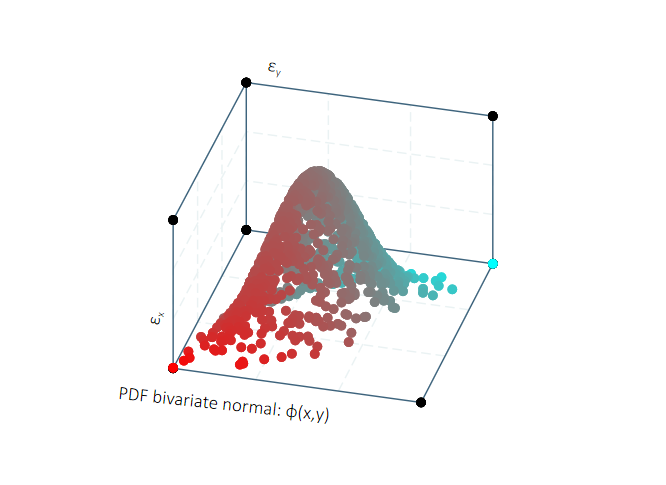
\includegraphics[width=0.45\textwidth]{figures/bivariate_normal_pdf.png}
		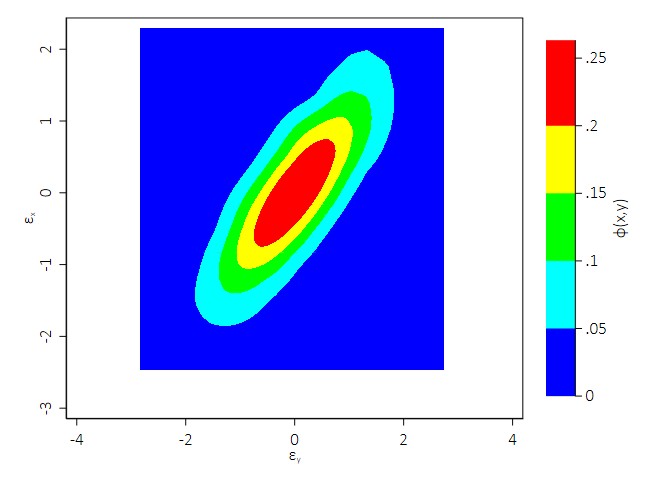
\includegraphics[width=0.45\textwidth]{figures/bivariate_normal_pdf_contour.png}
	\label{fig:bivariate_normal_pdf}
\end{figure}

\end{frame}


\section{The joint cumulative density function}
\begin{frame}{The joint cumulative density function}
\renewcommand{\baselinestretch}{1.45}
\footnotesize
The probability of a joint event of $X$ and $Y$ have $\textbf{joint cumulative density function}$
\begin{itemize}
	\item if $x$ and $y$ are discrete
$$F(x, y) =Prob(X \leq x, Y \leq y) = \sum_{X\leq x}\sum_{Y\leq y}f(x, y)$$
	\item if $x$ and $y$ are continuous
$$F(x, y) =Prob(X \leq x, Y \leq y)  = \int_{-\infty}^{x}\int_{-\infty}^{y}f(t, s)dsdt$$

\end{itemize}
\begin{example} 
\scriptsize
\renewcommand{\baselinestretch}{1}
With $x=2,y=2$ and the following $f(x,y)$\\
\newlength\Colsep
\setlength\Colsep{10pt}
\vspace{-3mm}

\noindent\begin{minipage}{\textwidth}
\vspace{-13mm}
\begin{minipage}[c][6cm][c]{\dimexpr0.5\textwidth-0.5\Colsep\relax}
%-------------------------------------------
%\begin{landscape}
\renewcommand{\baselinestretch}{1}
	\begin{center}
		\begin{threeparttable}[htbp]
%\caption{Timeline of German Reforms}
\label{tab:timeline}
\tiny
		\begin{tabular}{lrr}
\toprule
$f(x,y)$ &$f(x,y=1)$ &$f(x,y=2)$      \\
\midrule
$f(x=1,y)$ &\cellcolor{lightblue}1/10  &\cellcolor{lightblue}2/10                                                                 \\
$f(x=2,y)$ &\cellcolor{lightblue}1/10  &\cellcolor{lightblue}2/10                                                              \\
$f(x=3,y)$   &0     &4/10                                                             \\
\bottomrule
		\end{tabular}
		%\begin{tablenotes}
			%\item \emph{Notes:} We report the most important reforms of policies which affected pharmacies. The upper part of the table provides an overview of the historical development of the regulatory measures. The lower part provides the most important regulatory changes and announcements within our observation period. \newline
%\emph{Sources:} Own description.
		%\end{tablenotes}
	\end{threeparttable}
\end{center}
\renewcommand{\baselinestretch}{1.45}
%\end{landscape}
%-------------------------------------------
\tiny
$Prob(X \leq 2 , Y \leq 2)=f(x=1, y=1)+$\\$f(x=2, y=1)+f(x=1, y=2)+f(x=2, y=2)=3/5.$

\end{minipage}\hfill
\begin{minipage}[c][6cm][c]{\dimexpr0.5\textwidth-0.5\Colsep\relax}
\begin{figure}
	\centering
		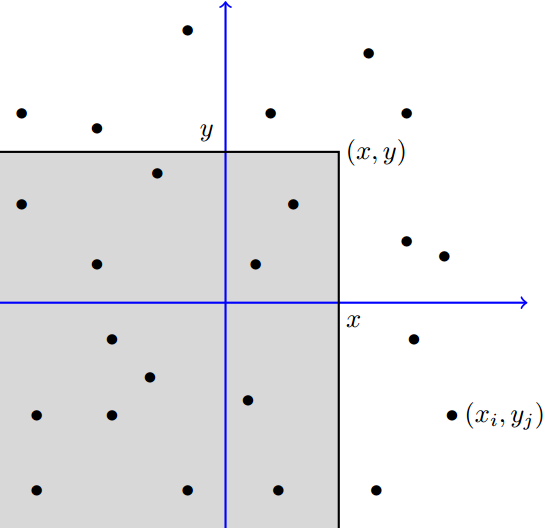
\includegraphics[width=0.50\textwidth]{figures/jointcdf.png}
	\label{fig:jointcdf}
\end{figure}
\end{minipage}%
\end{minipage}
\end{example}

\end{frame}


\begin{frame}{Bivariate probabilities}
For values $x$ and $y$ of two discrete random variable $X$ and $Y$, the \textbf{cumulative probability distribution}
$$F(x,y)=Prob(X\leq x,Y\leq y).$$
The axioms of probability require
$$0\leq F(x,y)\leq1,$$
$$F(\infty,\infty)=1,$$
$$F(-\infty,y)=0,$$
$$F(x,-\infty)=0.$$
The marginal probabilities can be found from the joint cdf
$$f_x(x)=P(X\leq x)=Prob(X\leq x,Y\leq \infty)=F(x,\infty).$$
\end{frame}


\section{The marginal probability density}
\begin{frame}{The marginal probability density}
\renewcommand{\baselinestretch}{1.45}
\footnotesize
To obtain the marginal distributions $f_x(x)$ and $f_y(y)$ from the joint density $f(x,y)$, it is necessary to sum or integrate out the other variable.
For example,
\begin{itemize}
	\item if $x$ and $y$ are discrete
$$f_{x}(x)=\sum_{y}f(x, y),$$
	\item if $x$ and $y$ are continuous
$$f_{x}(x)=\int_{y}f(x, s)ds.$$
\end{itemize}

\begin{example}
\scriptsize
\renewcommand{\baselinestretch}{1}
\vspace{-5mm}
%-------------------------------------------
%\begin{landscape}
\renewcommand{\baselinestretch}{1}
	\begin{center}
		\begin{threeparttable}[htbp]
%\caption{Timeline of German Reforms}
\label{tab:timeline}
\tiny
		\begin{tabular}{lrrr}
\toprule
$f(x,y)$ &$f(x,y=1)$ &$f(x,y=2)$ & $f_x(x)$     \\
\midrule
$f(x=1,y)$ &\cellcolor{lightblue}1/10  &\cellcolor{lightblue}2/10          &\cellcolor{lightblue}\Circled[outer color=persianred, inner ysep=3pt]{3/10}                                                          \\
$f(x=2,y)$ &1/10  &2/10          &3/10                                                       \\
$f(x=3,y)$   &0     &4/10        &4/10                                                        \\
$f_y(y)$    &2/10  &8/10 &1\\
\bottomrule
		\end{tabular}
		%\begin{tablenotes}
			%\item \emph{Notes:} We report the most important reforms of policies which affected pharmacies. The upper part of the table provides an overview of the historical development of the regulatory measures. The lower part provides the most important regulatory changes and announcements within our observation period. \newline
%\emph{Sources:} Own description.
		%\end{tablenotes}
	\end{threeparttable}
\end{center}
\renewcommand{\baselinestretch}{1.45}
%\end{landscape}
%-------------------------------------------
\tiny
$$f_x(x=1)=f(x=1,y=1)+f(x=1,y=2)=3/10.$$
$$f_y(y=2)=f(x=1,y=2)+f(x=2,y=2)+f(x=3,y=2)=4/5.$$
\end{example}


\end{frame}


\begin{frame}{The bivariate normal distribution}
\begin{figure}
	\centering
		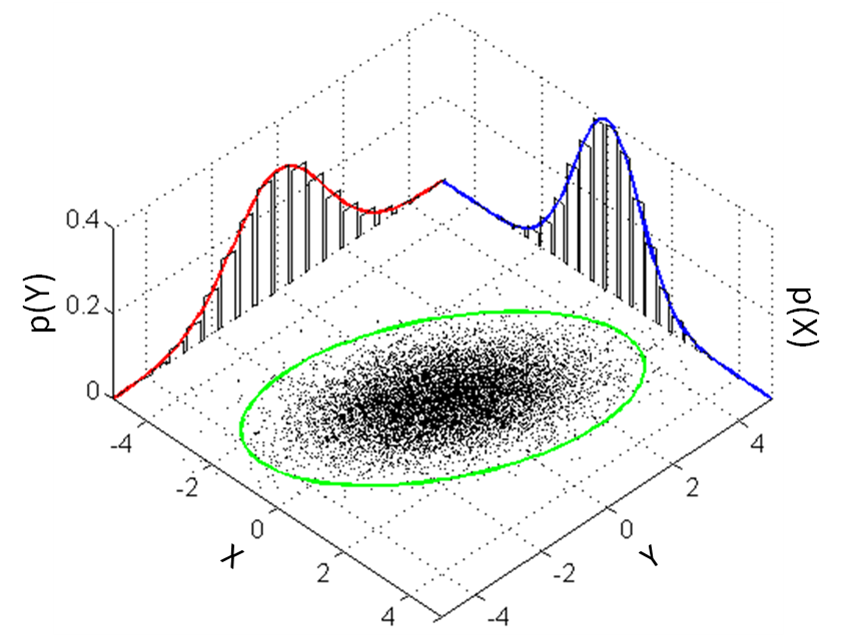
\includegraphics[width=0.70\textwidth]{figures/MultivariateNormal.png}
	\label{fig:MultivariateNormal}
\end{figure}

\end{frame}


\begin{frame}{Why do we care about marginal distributions?}
\renewcommand{\baselinestretch}{1.45}
Means, variances, and higher moments of the variables in a joint distribution are defined with respect to the marginal distributions.

\begin{itemize}
	\item \textbf{Expectations}\\
	If $x$ and $y$ are discrete
$$E[x] = \sum_{x}x f_{x}(x) =\sum_{x}x\left[\sum_{y}f(x, y)\right] = \sum_{x}\sum_{y} x f(x, y).$$
	If $x$ and $y$ are continuous
$$E[x] = \int_{x}x f_{x}(x) = \int_{x}\int_{y} x f(x, y)dydx.$$
	\item \textbf{Variances}
$$  Var[x] = \sum_{x}(x-E[x])^{2} f_{x}(x) = \sum_{x}\sum_{y} (x-E[x])^{2} f(x, y).$$

\end{itemize}
\end{frame}


\section{Covariance and correlation}
\begin{frame}{Covariance and correlation}
\renewcommand{\baselinestretch}{1.45}
\scriptsize For any function $g(x, y)$,
\begin{equation} E[g(x, y)]=\left\{
 \begin{array}{ll}
 {\sum_{x}\sum_{y}g(x, y)f(x, y)~~~~~~~~~ in~ the~ discrete~case, } \\
 {~}\\
 {\int_{x}\int_{y}g(x, y)f(x, x)dydx~~~~~~~ in~ the~ continuous~case.}
 \end{array}
 \right.
\end{equation}
The covariance of $x$ and $y$ is a special case:
\begin{eqnarray*}
% \nonumber to remove numbering (before each equation)
  Cov[x, y] &=& E[(x - \mu_{x})(y - \mu_{y})] \\
  ~ &=& E[xy] - \mu_{x}\mu_{y} = \sigma_{xy}
\end{eqnarray*}
If $x$ and $y$ are independent, then $f(x, y) = f_{x}(x) f_{y}(y)$ and
\begin{eqnarray*}
% \nonumber to remove numbering (before each equation)
  \sigma_{xy} &=& \sum_{x}\sum_{y}f_{x}(x)f_{y}(y)(x-\mu_{x})(y-\mu_{y}) \\
  ~ &=& \sum_{x}(x-\mu_{x})f_{x}(x)\sum_{y}(y-\mu_{y})f_{y}(y) = E[x-\mu_{x}]E[y-\mu_{y}]= 0.
\end{eqnarray*}
\vspace{-5mm}
\begin{itemize}
	\item correlation $\rho_{xy}=\frac{\sigma_{xy}}{\sigma_{x}\sigma_{y}}$
  \item $\sigma_{xy}=0$ does not imply independence (except for bivariate normal). 
\end{itemize}
\end{frame}



\begin{frame}{\small Independence: Pdf and cdf from marginal densities}
\renewcommand{\baselinestretch}{1.45}
\footnotesize
\begin{itemize}
	\item Two random variables are statistically independent if and only if their joint density is the product of the marginal densities:
$$f(x, y) = f_{x}(x) f_{y}(y) \Leftrightarrow x~ and~ y~ are~ independent.$$
	\item If (and only if) $x$ and $y$ are independent, then the marginal cdfs factors the cdf as well:
$$F(x, y) = F_{x}(x)F_{y}(y)=Prob(X \leq x, Y \leq y) = Prob(X \leq x)Prob(Y \leq y).$$
\end{itemize}

\begin{example}
\scriptsize

\setlength\Colsep{10pt}

\noindent\begin{minipage}{\textwidth}
\vspace{-10mm}
\begin{minipage}[c][6cm][c]{\dimexpr0.5\textwidth-0.5\Colsep\relax}
\vspace{-10mm}
\renewcommand{\baselinestretch}{1}
%-------------------------------------------
%\begin{landscape}
\renewcommand{\baselinestretch}{1}
	\begin{center}
		\begin{threeparttable}[htbp]
%\caption{Timeline of German Reforms}
\label{tab:timeline}
\tiny
		\begin{tabular}{lrrr}
\toprule
$f(x,y)$ &$f(x,y=1)$ &$f(x,y=2)$ & $f_x(x)$     \\
\midrule
$f(x=1,y)$ &1/6  &1/6          &1/3                                                          \\
$f(x=2,y)$ &1/6  &1/6          &1/3                                                       \\
$f(x=3,y)$ &1/6  &\Circled[outer color=persianred, inner ysep=3pt]{1/6}          &\cellcolor{lightblue}1/3                                                        \\
$f_y(y)$   &1/2  &\cellcolor{lightblue}1/2 &1\\
\bottomrule
		\end{tabular}
		%\begin{tablenotes}
			%\item \emph{Notes:} We report the most important reforms of policies which affected pharmacies. The upper part of the table provides an overview of the historical development of the regulatory measures. The lower part provides the most important regulatory changes and announcements within our observation period. \newline
%\emph{Sources:} Own description.
		%\end{tablenotes}
	\end{threeparttable}
\end{center}
\renewcommand{\baselinestretch}{1.45}
%\end{landscape}
%-------------------------------------------
\tiny
$$f_x(x=3)\times f_y(y=2)=1/3\times 1/2=1/6.$$

\end{minipage}\hfill
\begin{minipage}[c][6cm][c]{\dimexpr0.5\textwidth-0.5\Colsep\relax}
\renewcommand{\baselinestretch}{1}
%-------------------------------------------
%\begin{landscape}
\renewcommand{\baselinestretch}{1}
	\begin{center}
		\begin{threeparttable}[htbp]
%\caption{Timeline of German Reforms}
\label{tab:timeline}
\tiny
		\begin{tabular}{lrrr}
\toprule
$F(x,y)$ &$F(x,y=1)$ &$F(x,y=2)$      \\
\midrule
$F(x=1,y)$ &1/6  &\cellcolor{lightblue}2/6                                                                  \\
$F(x=2,y)$ &\cellcolor{lightblue}2/6  &4/6                                                               \\
$F(x=3,y)$ &3/6  &1                                                                  \\
\bottomrule
		\end{tabular}
		%\begin{tablenotes}
			%\item \emph{Notes:} We report the most important reforms of policies which affected pharmacies. The upper part of the table provides an overview of the historical development of the regulatory measures. The lower part provides the most important regulatory changes and announcements within our observation period. \newline
%\emph{Sources:} Own description.
		%\end{tablenotes}
	\end{threeparttable}
\end{center}
\renewcommand{\baselinestretch}{1.45}
%\end{landscape}
%-------------------------------------------
\tiny
$$P(x\leq2)P(y\leq2)=[f(x=2,y=1)+f(x=2,y=2)]\times$$
$$[f(x=1,y=2)+f(x=2,y=2)]$$
$$=[1/6+1/6][1/6+1/6]=4/36=2/18.$$

\end{minipage}%
\end{minipage}

\end{example}
\end{frame}



\section{The conditional density function}
\begin{frame}{The conditional density function}
\renewcommand{\baselinestretch}{1.45}
\scriptsize
The $\textbf{conditional distribution}$ over $y$ for each value of $x$ (and vice versa) has
conditional densities
 $$f(y | x) = \frac{f(x, y)}{f_{x}(x)} \quad	 f(x | y) = \frac{f(x, y)}{f_{y}(y)}.$$
The marginal distribution of $x$ averages the probability of $x$ given $y$ over the distribution of all values of $y$
$f_x(x)=E[f(x|y)f(y)].$ If $x$ and $y$ are independent, knowing the value of $y$ does not provide any information about $x$, so $f_x(x)=f(x|y).$ 

\begin{example}
\vspace{-5mm}
%-------------------------------------------
%\begin{landscape}
\renewcommand{\baselinestretch}{1}
	\begin{center}
		\begin{threeparttable}[htbp]
%\caption{Timeline of German Reforms}
\label{tab:timeline}
\tiny
		\begin{tabular}{l@{\extracolsep{-2mm}}rrrr@{\extracolsep{0pt}}l@{\extracolsep{-2mm}}rrr}
\cmidrule(r){1-4}\cmidrule(r){6-9}
cond. distr.  &  & &  &	 &	joint distr.  &  &  &marginal pr.     \\
 $f(x|y)$ &$f(x|y=1)$ &$f(x|y=2)$ &$f(x|y=1,y=2)$ & &	$f(x,y)$ &$f(x,y=1)$ &$f(x,y=2)$  &  $f_x(x)$    \\
\cmidrule(r){1-4}\cmidrule(r){6-9}
$x=1$ &1/2  &1/4 &3/10 & &	$f(x=1,y)$ &1/10  &2/10 &3/10                                                                \\
$x=2$ &1/2  &1/4 &3/10 & &	$f(x=2,y)$ &1/10  &2/10 &3/10                                                             \\
$x=3$ &0  &\Circled[outer color=persianred, inner ysep=3pt]{1/2} &4/10 & &	$f(x=3,y)$   &0     &\cellcolor{lightblue}4/10 &4/10                                                             \\
$\sum_x $ &1 &1  &1 &	& marginal pr. $f_y(y)$    &2/10  &\cellcolor{lightblue}8/10 &1                                            \\
\cmidrule(r){1-4}\cmidrule(r){6-9}
\end{tabular}
		%\begin{tablenotes}
			%\item \emph{Notes:} We report the most important reforms of policies which affected pharmacies. The upper part of the table provides an overview of the historical development of the regulatory measures. The lower part provides the most important regulatory changes and announcements within our observation period. \newline
%\emph{Sources:} Own description.
		%\end{tablenotes}
	\end{threeparttable}
\end{center}
\renewcommand{\baselinestretch}{1.45}
%\end{landscape}
%-------------------------------------------
\tiny
$$f(x=3|y=2)=\frac{f(x=3,y=2)}{f_y(y=2)}=4/10\times 10/8=1/2.$$
$$f_x(x=2)=E_y[f(x=2|y)f(y)]=f(x=2|y=1)f(y=1)+f(x=2|y=2)f(y=2)$$
$$=1/2\times2/10+1/4\times8/10=1/10+2/10=3/10.$$

\end{example}

\end{frame}

\section{Conditional mean aka regression}

\begin{frame}{Conditional mean aka regression}
\renewcommand{\baselinestretch}{1.45}
A random variable may always be written as
\begin{eqnarray*}
% \nonumber to remove numbering (before each equation)
  y &=& E[y | x] + (y - E[y | x]) \\
  ~ &=& E[y | x] + \epsilon.
\end{eqnarray*}


\begin{definition}
The regression of $y$ on $x$ is obtained from the $\textbf{conditional mean}$
\begin{equation} E[y | x]=\left\{
 \begin{array}{ll}
 {\sum_{y}yf(y | x) ~~~~~~~ if~ y~ is~ discrete,}\\
 {~}\\
 {\int_{y}yf(y | x)dy~~~~~~~ if ~y~is~ continuous.} 
 \end{array}
 \right.
\end{equation}
\end{definition}
\end{frame}



\begin{frame}{Conditional mean aka regression}
\renewcommand{\baselinestretch}{1.45}
\footnotesize
Predict $y$ at values of $x$: $$\sum_{y}yf(y | x=1)=1\times 1/3+2\times 2/3=5/3.$$
\begin{figure}
	\centering
		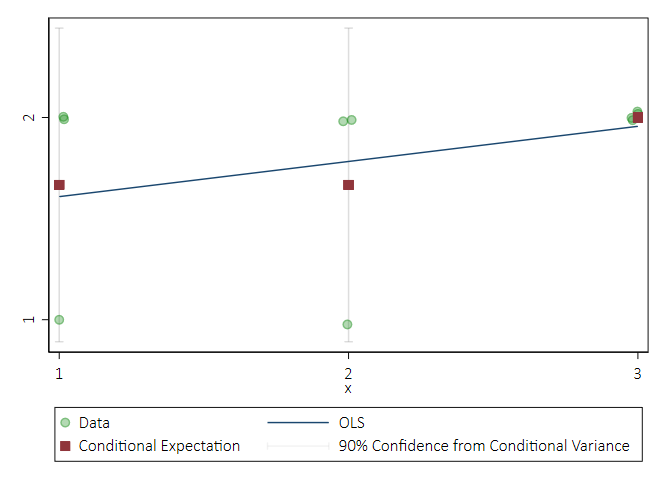
\includegraphics[width=0.50\textwidth]{figures/conditional_expectation.png}
	\label{fig:conditional_expectation}
\end{figure}


\end{frame}


\begin{frame}{Conditional variance}
\renewcommand{\baselinestretch}{1.45}
A $\textbf{conditional variance}$ is the variance of the conditional distribution:
{\small{\begin{equation} Var[y | x] =\left\{
 \begin{array}{ll}
 {\sum_{y}\left(y - E[y | x]\right)^{2}f(y | x) ~~~~~~~ if~ y~ is~ discrete,} \\
 {~}\\
 {\int_{y}\left(y - E[y | x]\right)^{2}f(y | x) dy,~~~~~ if ~y~is~ continuous. } 
 \end{array}
 \right.
\end{equation}}}
The computation can be simplified by using
\begin{equation}
    Var[y | x] = E[y^{2} | x] - \left(E[y | x]\right)^{2}\geq0.
\end{equation}
Decomposition of variance $Var[y] = E_{x}[Var[y | x]]+Var_{x}[E[y | x]]$
\begin{itemize}
	\item When we condition on $x$, the variance of $y$ reduces on average. $Var[y]\geq E_{x}[Var[y | x]]$
	\item $E_{x}[Var[y | x]]$ is the average of variances \textbf{within} each $x$
	\item $Var_{x}[E[y | x]]$ is variance \textbf{between} $y$ averages in each $x$. 
\end{itemize}
\end{frame}



\begin{frame}{Conditional expectations and variances}
\renewcommand{\baselinestretch}{1.45}
\footnotesize
\begin{itemize}
	\item $E[y|x=1]=1.67$, $E[y|x=2]=1.67$, and $E[y|x=3]=2$
	\item $V[y|x=1]=0.22$, $V[y|x=2]=0.22$, and $V[y|x=3]=0$
\end{itemize}

\begin{example}
\scriptsize

\setlength\Colsep{10pt}

\noindent\begin{minipage}{\textwidth}
\vspace{-5mm}
\begin{minipage}[c][6cm][c]{\dimexpr0.5\textwidth-0.5\Colsep\relax}
\vspace{-10mm}
\renewcommand{\baselinestretch}{1}
%-------------------------------------------
%\begin{landscape}
\renewcommand{\baselinestretch}{1}
	\begin{center}
		\begin{threeparttable}[htbp]
%\caption{Timeline of German Reforms}
\label{tab:timeline}
\tiny
		\begin{tabular}{lrrr}
\toprule
$f(y|x)$ &$y=1$ &$y=2$      \\
\midrule
$f(y|x=1)$ &1/3  &2/3          &1                                                          \\
$f(y|x=2)$ &1/3  &2/3          &1                                                       \\
$f(y|x=3)$ & 0  &1           &1                                                       \\
\bottomrule
		\end{tabular}
		%\begin{tablenotes}
			%\item \emph{Notes:} We report the most important reforms of policies which affected pharmacies. The upper part of the table provides an overview of the historical development of the regulatory measures. The lower part provides the most important regulatory changes and announcements within our observation period. \newline
%\emph{Sources:} Own description.
		%\end{tablenotes}
	\end{threeparttable}
\end{center}
\renewcommand{\baselinestretch}{1.45}
%\end{landscape}
%-------------------------------------------
\tiny
$$E[y|x=1]=1/3\times1+2/3\times 2=5/3$$
$$E[y|x=2]=1/3\times1+2/3\times 2=5/3$$
$$E[y|x=3]=0\times1+1\times 2=2$$

\end{minipage}\hfill
\begin{minipage}[c][6cm][c]{\dimexpr0.5\textwidth-0.5\Colsep\relax}
\renewcommand{\baselinestretch}{1}
%-------------------------------------------
%\begin{landscape}
\renewcommand{\baselinestretch}{1}
	\begin{center}
		\begin{threeparttable}[htbp]
%\caption{Timeline of German Reforms}
\label{tab:timeline}
\tiny
		\begin{tabular}{lrrr}
\toprule
$f(x,y)$ &$f(x,y=1)$ &$f(x,y=2)$ & $f_x(x)$     \\
\midrule
$f(x=1,y)$ &1/10  &2/10 & 3/10                                                                 \\
$f(x=2,y)$ &1/10  &2/10 & 3/10                                                               \\
$f(x=3,y)$ &0     &4/10 & 4/10                                                       \\
$f_y(y)$   &2/10  &8/10 & 1                                                                \\
\bottomrule
		\end{tabular}
		%\begin{tablenotes}
			%\item \emph{Notes:} We report the most important reforms of policies which affected pharmacies. The upper part of the table provides an overview of the historical development of the regulatory measures. The lower part provides the most important regulatory changes and announcements within our observation period. \newline
%\emph{Sources:} Own description.
		%\end{tablenotes}
	\end{threeparttable}
\end{center}
\renewcommand{\baselinestretch}{1.45}
%\end{landscape}
%-------------------------------------------
\tiny
$$V[y|x=1]=1^2\times 1/3+2^2\times 2/3-(5/3)^2=2/9$$
$$V[y|x=2]=1^2\times 1/3+2^2\times 2/3-(5/3)^2=2/9$$
$$V[y|x=3]=1^2\times 0+2^2\times 1-2^2=0$$
alternatively (requiring more differences)
$$V[y|x=1]=(1-5/3)^2\times 1/3+(2-5/3)^2\times 2/3=2/9$$

\end{minipage}%
\end{minipage}

\end{example}
\end{frame}



\begin{frame}{Conditional expectations and variances}
\renewcommand{\baselinestretch}{1.45}
\scriptsize
Average of variances \textbf{within} each $x$, $E[V[y|x]]$ is less or equal total variance $V[y]$.
\begin{example}
\tiny

\begin{itemize}
	\item Use the conditional mean to calculate $E[y]$:
$$E[y]=E_x[E[y|x]]=E[y|x=1]f(x=1)+E[y|x=2]f(x=2)+E[y|x=3]f(x=3)$$$$=5/3\times 3/10+5/3\times 3/10+2\times 4/10=9/5.$$
$$E[y]=\sum_yf_y(y)=1\times 2/10+2\times 8/10=9/5.$$
	\item Variation in $y$, $V[y|x=1]=0.22$, $V[y|x=2]=0.22$, and $V[y|x=3]=0$ due to variation in $x$, is on average\\ $E[V[y|x]]=3/10\times2/9+3/10\times2/9+4/10\times0=2/15.$
  \item For each conditional mean $E[y|x=1]=5/3$, $E[y|x=2]=5/3$, and $E[y|x=3]=2$, $y$ varies with\\
	$V[E[y|x]]=E[(E[y|x])^2]-(E[y|x])^2=3/10\times(5/3)^2+3/10\times(5/3)^2+4/10\times(2)^2-(9/5)^2=2/75.$
	\item $E[V[y|x]]+V[E[y|x]]=V[y]=2/75+2/15=4/25.$\\
With degree of freedom correction $(n-1)$ (as reported in software):\\
$E[V[y|x]]+V[E[y|x]]=V[y]=2/75/(10-1)\times 10+2/15/(10-1)\times 10=8/45.$
\end{itemize}


\end{example}
\end{frame}


\section{The bivariate normal}
\begin{frame}{Properties of the bivariate normal}
\renewcommand{\baselinestretch}{1.45}

Recall bivariate normal distribution is the joint distribution of two normally distributed variables. The density is
\begin{equation}
    f(x, y) =\frac{1}{2\pi\sigma_{x}\sigma_{y}\sqrt{1 - \rho^{2}}}e^{-1/2[(\epsilon^{2}_{x}+\epsilon^{2}_{y}-2\rho \epsilon_{x} \epsilon_{y})/(1-\rho^{2})],}
\end{equation}
where $\epsilon_{x} = \frac{x - \mu_{x}}{\sigma_{x}},$ and $\epsilon_{y} = \frac{y - \mu_{y}}{\sigma_{y}}.$

The covariance is $\sigma_{xy}=\rho_{xy}\sigma_{x}\sigma_{y},$ where
\begin{itemize}
	\item $-1<\rho_{xy}<1$ is the correlation between $x$ and $y$
	\item $\mu_x,\sigma_{x},\mu_y,\sigma_{y}$ are means and standard deviations of the marginal distributions of $x$ or $y$
\end{itemize}
\end{frame}


\begin{frame}{Properties of the bivariate normal}
\renewcommand{\baselinestretch}{1.45}

If $x$ and $y$ are bivariately normally distributed $(x,y)\sim N_2[\mu_x,\mu_y,\sigma^2_{x},\sigma^2_{y},\rho_{xy}]$
\begin{itemize}
	\item the marginal distributions are normal $$f_x(x)=N[\mu_x,\sigma_x^2]$$$$f_y(y)=N[\mu_y,\sigma_y^2]$$
	\item the conditional distributions are normal $$f(y|x)=N[\alpha + \beta x, \sigma_y^2(1-\rho^2)]$$ $$\alpha=\mu_y-\beta \mu_x; \beta=\frac{\sigma_{xy}}{\sigma^2_{x}}$$ 
	\item $f(x,y)=f_x(x)f_x(x)$ if $\rho_{xy}=0$: $x$ and $y$ are independent if and only if they are uncorrelated
\end{itemize}
\end{frame}

\section{Useful rules}
\begin{frame}{Useful rules}
\renewcommand{\baselinestretch}{1.45}

\begin{itemize}
	\item $\rho_{xy}=\frac{\sigma_{xy}}{\sigma_{x}\sigma_{y}}$
	\item $E[ax + by + c] = aE[x] + bE[y] + c$
	\item $Var[ax + by + c] = a^{2}Var[x] + b^{2}Var[y] + 2abCov[x, y]=Var[ax + by]$
	\item $Cov[ax + by, cx + dy] = ac Var[x] + bd Var[y] + (ad + bc)Cov[x, y]$
	\item If $X$ and $Y$ are uncorrelated, then $Var[x + y] = Var[x - y] = Var[x] + Var[y].$
\end{itemize}
\renewcommand{\baselinestretch}{1}

\end{frame}


\begin{frame}{Useful rules}
\renewcommand{\baselinestretch}{1.45}
\small
\begin{itemize}
	\item Linearity
	$$E[ax + by |z] = aE[x|z] + bE[y|z].$$
	\item Adam's Law / Law of Iterated Expectation
	$$E[y] = E_{x}[E[y | x]]$$
	\item Adam's general Law / Law of Iterated Expectation
	$$E[y|g_{2}(g_{1}(x))] = E[E[y | g_{1}(x)]|g_{2}(g_{1}(x))]$$
	\item Independence\\
	If $x$ and $y$ are independent, then $$E[y] = E[y|x],$$
	$$E[g_{1}(x)g_{2}(y)] = E[g_{1}(x)]E[g_{2}(y)].$$
	

\end{itemize}
\renewcommand{\baselinestretch}{1}

\end{frame}


\begin{frame}{Useful rules}
\renewcommand{\baselinestretch}{1.45}
\small

\begin{itemize}

	\item Taking out what is known
	$$E[g_{1}(x)g_{2}(y)|x] = g_{1}(x)E[g_{2}(y)|x].$$
	\item Projection of $y$ by $E[y|x]$, such that orthogonal to $h(x)$
	$$E[(y-E[y|x])h(x)] = 0.$$
	\item Keeping just what is needed ($y$ predictable from $x$ needed, not residual)
	$$E[xy] = E[xE[y|x]].$$
	\item Eve's Law (EVVE) / Law of Total Variance
	$$Var[y] = E_{x}[Var[y | x]] + Var_{x}[E[y | x]]$$
	\item ECCE law / Law of Total Covariance
	$$Cov[x,y] = E_{z}[Cov[y,x | z]] + Cov_{z}[E[x | z],E[y | z]]$$

\end{itemize}
\renewcommand{\baselinestretch}{1}

\end{frame}

\begin{frame}{Useful rules}
\renewcommand{\baselinestretch}{1.45}

\begin{itemize}
	\item $Cov[x, y] = Cov_{x}[x, E[y | x]] =\int_{x}\left(x - E[x]\right)E[y | x] f_{x}(x) dx.$
	\item If $E[y | x] = \alpha + \beta x$, then $\alpha = E[y] - \beta E[x]$ and $\beta= \frac{Cov[x, y]}{Var[x]}$
	\item Regression variance $Var_{x}[E[y | x]]$, because $E[y | x]$ varies with $x$
	\item Residual variance $E_{x}[Var[y | x]] = Var[y] - Var_{x}[E[y | x]]$, because $y$ varies around the conditional mean
	\item Decomposition of variance $Var[y] = Var_{x}[E[y | x]] + E_{x}[Var[y | x]]$
	\item Coefficient of determination $= \frac{\text{regression~ variance}}{\text{total variance}}$
	\item If $E[y | x] = \alpha + \beta x$ and if $Var[y | x]$ is a constant, then $$Var[y | x] = Var[y]\left(1 - Corr^{2}[y, x]\right)= \sigma^{2}_{y}\left(1 - \sigma^{2}_{xy}\right)$$
\end{itemize}
\renewcommand{\baselinestretch}{1}

\end{frame}




\begin{frame}[t,allowframebreaks
]\nocite{*}
\frametitle{References}
\small
\bibliography{bib}
\end{frame}


\end{document}
